\chapterauthor{Hein-Erik Schnell}
This section is divided into the three crucial tasks for which we needed to develop a concept in order to get the agent into training. Those tasks were:

\begin{itemize}
	\item Choosing a suitable \textit{state representation} to be then passed to an \textit{regressor} to estimate the expected \textit{reward} for each of the possible actions
	\item Choosing suitable \textit{rewards} in order to communicate the goals of the game to the agent
	\item Choosing a suitable \textit{regressor} which estimates the expected \textit{reward} for each possible action at the current state of the game.
\end{itemize}

	\subsection{State representation}
	\chapterauthor{Hein-Erik Schnell}
	The first task was to choose a suitable state representation. In case of regressors provided by \textit{scikit-learn}, the training data is usually passed to the regressor as a 2D-array where each row (first index) represents a single state and each column (second index) represents a feature of the respective states. Analagously, the prediction then demands an array of similar form. The regressor then returns an array with as many predicted values as there were rows (states) in the input array. If one wants to predict only a single value, one may not pass a 1D-array to the regressor but create an additional dummy dimension. All this means that if we want to use precoded regressors from scikit-learn, we need to find a 1D-array representation for a single state. \par
	
	After each step, the relevant data is passed to the agent via the dictionary \code{self.game\_state}. In the agents \code{callbacks.py} we defined the function \code{create\_state\_vector(\textit{self})} which turns the information provided by \code{self.game\_state} into a 1D-array. We chose to store the relevant features in the following way:
	
	\subsubsection{State representation 1}
	\label{State_rep_1}
	\begin{itemize}
		\item For each cell:
		\begin{itemize}
			\item \textbf{Agent, Opponent, None \state{1,-1,0}}:\\
			The dictionary provides the entry \code{self.game\_state['arena']} which is a 2D representation of the game board. We use this to create a numpy-array \code{agent\_state} of the same shape which is $1$ on the agents position, $-1$ on cells with an opponent and $0$ on all other cells.
			\item \textbf{Crate, Coin, Empty/Wall \state{-1,1,0}}: \\
			A copy of \code{self.game\_state['arena']} is manipulated in such a way that it is $-1$ for a crate, $1$ for a coin on the respective cell and $0$ in all other cases. This would mean that the agent could not distinguish between empty cells and walls. This issue is resolved later when we delete all cells which contain walls. These cells are always the same and therefore do not contribute to the learning process. In our code, this whole part is represented by the variable \code{loot\_state}.
			\item \textbf{Bombs} \state{6,5 \dots 2,1,0}:\\
			The variable \code{bomb\_state} is of the same shape as \code{self.game\_state['arena']}. All cells are by default $6$. If the cell will soon be affected by a bombs explosion, the values $5\dots2$ represent the 4-time-steps countdown. $1\dots0$ represent the 2-time-steps explosion. This way, \code{bomb\_state} provides a danger level for each cell. $6$ means no danger at all.
			
		\end{itemize}
		\item Just once (implemented in our code as \code{extras}):
		\begin{itemize}
			\item \textbf{Current step number \state{1,\dots,400}}:\\
			\code{extras[0]} contains the current time step.
			\item \textbf{Danger level} \state{0,\dots,6}:\\
			\code{extras[1]} represents the danger level on the agents current position. It is calculated by $6 - \text{\code{bomb\_state[x,y]}}$, where \code{x} and \code{y} are the coordinates of the agents position. Consequently, this danger level in invers to the danger level in \code{bomb\_state}, i.e. $0$ means no danger, $1\dots4$ means increasing danger and $5\dots6$ would be bombs exploding. The least point is rather irrelevant since the agent would already have been deleted by the environment.
			\item \textbf{Bomb action possible \state{0,1}}:\\
			\code{extras[2]} is $1$ if the agent could place a bomb and $0$ if not (i.e. if an own bomb is still ticking).
			\item \textbf{Touching opponent} \state{0,1}:\\
			\code{extras[3]} is $1$ if an opponent is on a neighbouring cell and $0$ if not.
		\end{itemize}
	\end{itemize}

	After manipulating the data in the described way, all cells containing walls are deleted from the 2D-arrays \code{agent\_state}, \code{loot\_state} and \code{bomb\_state}. As already described above, this is done because these entries will always be the same and therefore never contribute to the learning of the agent. The three arrays are then flattened and concatenated after one another into the 1D-array \code{vector}. Finally, we append the \code{extras} to the \code{vector}, which is then returned by the function \code{create\_state\_vector}.\par
	
	With the described representation of a state we combined features which could be represented as seperate features into single features. For example in \cite{paper}, each cell has a feature \textit{Agent on cell?} and \textit{Opponent on cell?} which can both assume the values $0$ and $1$. We combined these two features. As we see it, a proper regressor should be able to determine the important features as well as the relevant range of values of a feature. A \textit{Random Forest Regressor}, for instance, should theoretically be able to do so since the way it works is to find the most relevant feature and its most divisive value.\par
	
	With \textit{state representation 1} ($532$ features), the feature space has at most about $5.4 \times 10^{320}$ possible states. 
	% Calculated with 3^(17*17-34-30-49) * 3^(17*17-34-30-49) * 7^(17*17-34-30-49)*400*7*2*2
	
	\subsubsection{State representation 2}
	\label{State_rep_2}
	As described later in section \ref{results}, our agent never managed to get out of its starting corner. In order to change that, we condensed the above state vector ($532$ features) into a much smaller state vector of $180$ features. The main idea of this smaller state vector is that agents, opponents, crates and coins can never occupy the same cell. Bombs could occupy the same cell as agents, opponents or coins, but for the sake of the agent they shouldn't:
	
	\begin{itemize}
		\item For each cell:
		\begin{itemize}
			\item \textbf{Empty, agent, opponent, crate, coin, danger level} \state{0,1,2,4,5 \dots 11}:\\
			Empty cells are $0$. Cells with agent, opponent, crate or coin are \state{1,2,3,4}, respectively. The values \state{5 \dots 11} represent the danger level because there is a bomb affecting the respective cell. $5$ is not used, \state{6 \dots 9} is the four-time-steps countdown, \state{10,11} the two-time-steps explosion. If there is a danger level the values \state{1,2,3,4} are overwritten. This means that the position of the agent might not be represented anymore in this feature.
		\end{itemize}
		\item Just once (implemented in our code as \code{extras})
		\begin{itemize}
			\item \textbf{Danger level} \state{6 \dots 11}:\\ 
			\code{extras[0]} is the danger level at the position of the agent.
			\item \textbf{Bomb action possible} \state{0,1}: \\
			\code{extras[1]} is $1$ if the agent could place a bomb and $0$ if not (i.e. if an own bomb is still ticking).
			\item \textbf{Touching opponent} \state{0,1}: \\
			\code{extras[2]} is $1$ if an opponent is on a neighbouring cell and $0$ if not.
			\item \textbf{Position of agent} \state{18 \dots 271}: \\
			\code{extras[3]} is essentially the enumerated cell number of the agents position. It is calculated by $17x + y$, where $x$ and $y$ are the agents $x$- and $y$-coordinates. 
		\end{itemize} 
	\end{itemize}
	
	With \textit{state representation 2} (180 features) it has at most about $3.4 \times 10^{193}$ possible states, which is much less than with \textit{state representation 1}. For both representations, these are only upper limits. But both are calculated the same way so that these values are useful for comparisons between both representations.
	% Calculated with 12^(17*17-34-30-49) * 6 * 2 * 2 * (17*17-34-30-49)
	
	\subsection{Rewards}
	\chapterauthor{Karl Thyssen}
	The individual rewards for events that occur in a given step contribute to the reward function and are explicitly defined in the \code{reward\_update()} and \code{end\_of\_episode} functions. The other parameter to influence is the discount factor $\gamma$ for the discounted long term reward. We ran training with factors $\gamma = 1.0$ and $\gamma = 0.9$. The reward function is describe by a series of if clauses that determine the quality of the action taken and apply the reward.
\begin{itemize}
	\item \textbf{Valid move}: $-1$ \\Every step is punished in a small way to encourage the agent to complete tasks in the shortest possible time to avoid stacking negative rewards.
	\item \textbf{Wait}: $-5$\\We noticed while running preliminary quick trains that the agent quickly regressed into a pattern of repeated 'Waits' after only a few generations. Arguably other factors were also different at the time so its debatable how effective this now is.
	\item \textbf{Invalid action}: $-100$\\Invalid actions should be punished so the agent quickly learns the connections in between the fields and the restrictions on the frequency of bomb placements.
	\item \textbf{Destroy crate}: $+10$\\The agent should learn to destroy crates
	\item \textbf{Coin found}: $+20$\\The agent should want to destroy as many crates as possible to find coins
	\item \textbf{Collect coin}: $+2000$\\The agent is heavily rewarded for finding coins to incentivise coin collection as a primary goal 
	\item \textbf{Killed opponent}: $+10000$\\If the agent does accidentally kill an agent in training it should have a large weighting so this behaviour can be encouraged, particularly as this will be rare initially
	\item \textbf{Die (from opponent bomb)}: $-2000$\\The agent should learn to avoid all bombs...
	\item \textbf{Die (suicide)}: $-1500$\\...but rather die to its own to deny opponents 5 points.
\end{itemize}	
	
	\subsection{Regressors}
	\chapterauthor{Hein-Erik Schnell}
	In order to estimate the expected rewards properly we need to find a regressor which is both flexible and very decisive with respect to the features. Flexible, because a simple linear regressor would not be able to resemble the volume of states and outcomes. This big variety of possible states, even at the very beginning of an episode, means that many features are not relevant in a given situation. This is the reason why the regressor should also be able to find the most decisive features.\par
	
	Since we will not know whether the competition will be split into two leagues, one for neural networks and one for classical regressors, we initially decided to train both a classical regressor and a neural network and see which one performs better (in its respective league).\par
	
	As a classical model we chose to use a \textit{Random Forest Regressor}. The advantage of this regressor is that it is infinitely flexible can and can cope with whatever shape the reward function may assume. However, it turns out that this regressor is also quite inaccurate and erratic. Its erratic nature might be problematic because the order of the estimated rewards, i.e. which move is the best, is very important. If the order can not be predicted correctly the agent will not choose the best but only a good move. Figure \ref{forest_mlp_comp2} shows how likely this is. We chose to use the Random Forest Regressor provided by \textit{scikit-learn}.\par
	
	As a neural network we chose the \textit{MLP-Regressor} provided by \textit{scikit-learn} mainly for two reasons. The first reason is that we need a precoded regressor since neural networks haven't been subject to the lecture yet. The other reason is that the syntax and available functions of that regressor are the same as for the Random Forest Regressor. This way we only need to change the initialization of our regressor and do not have to change the rest of the code. It is basically changing one line of the code in order to switch between both regressors.\par
	
	The two regressors are initialized as follows:
	\begin{itemize}
		\item \code{RandomForestRegressor()}
		\item \code{MLPRegressor(max\_iter=500)}
	\end{itemize}
	Thus, we used the Forest with its default settings and changed the maximum number of iterations of the MLP to $500$ (default is $200$).
	
	\begin{figure}[h]
		\centering
		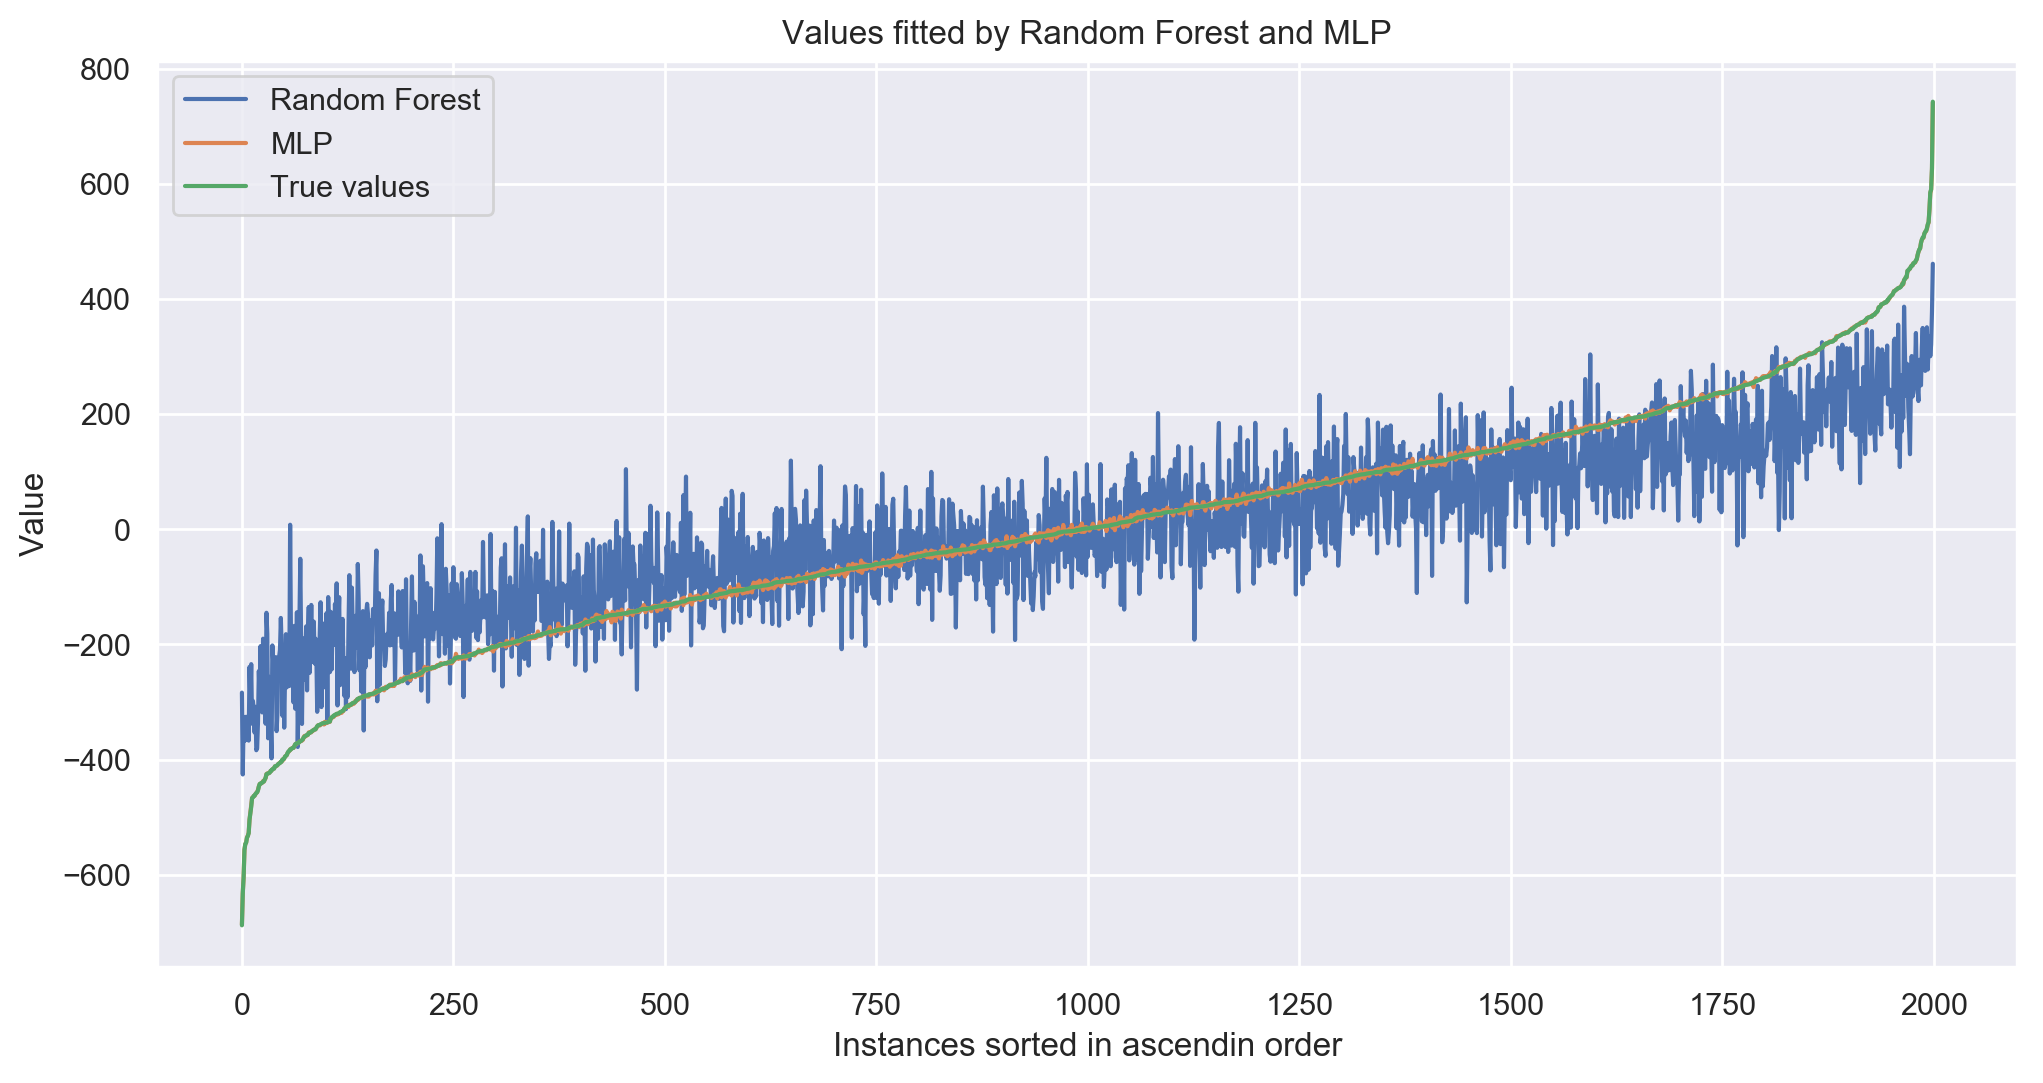
\includegraphics[width=\linewidth]{images/mlp_forest_comparison01.png}
		\caption{\textit{For this figure, {\normalfont \code{sklearn.datasets.make\_regression}} was used to create $10000$ samples with $100$ features of which $10$ are informative. We then trained the Random Forest Regressor and the MLP-Regressor provided by {\normalfont scikit-learn} with $80\%$ of the generated data. The figure shows the predicted values of the remaining $20\%$ of the data which were used as a test set. The test set has previously been sorted by the true target value in ascending order.}}
		\label{forest_mlp_comp1}
	\end{figure}
	\begin{figure}[h]
		\centering
		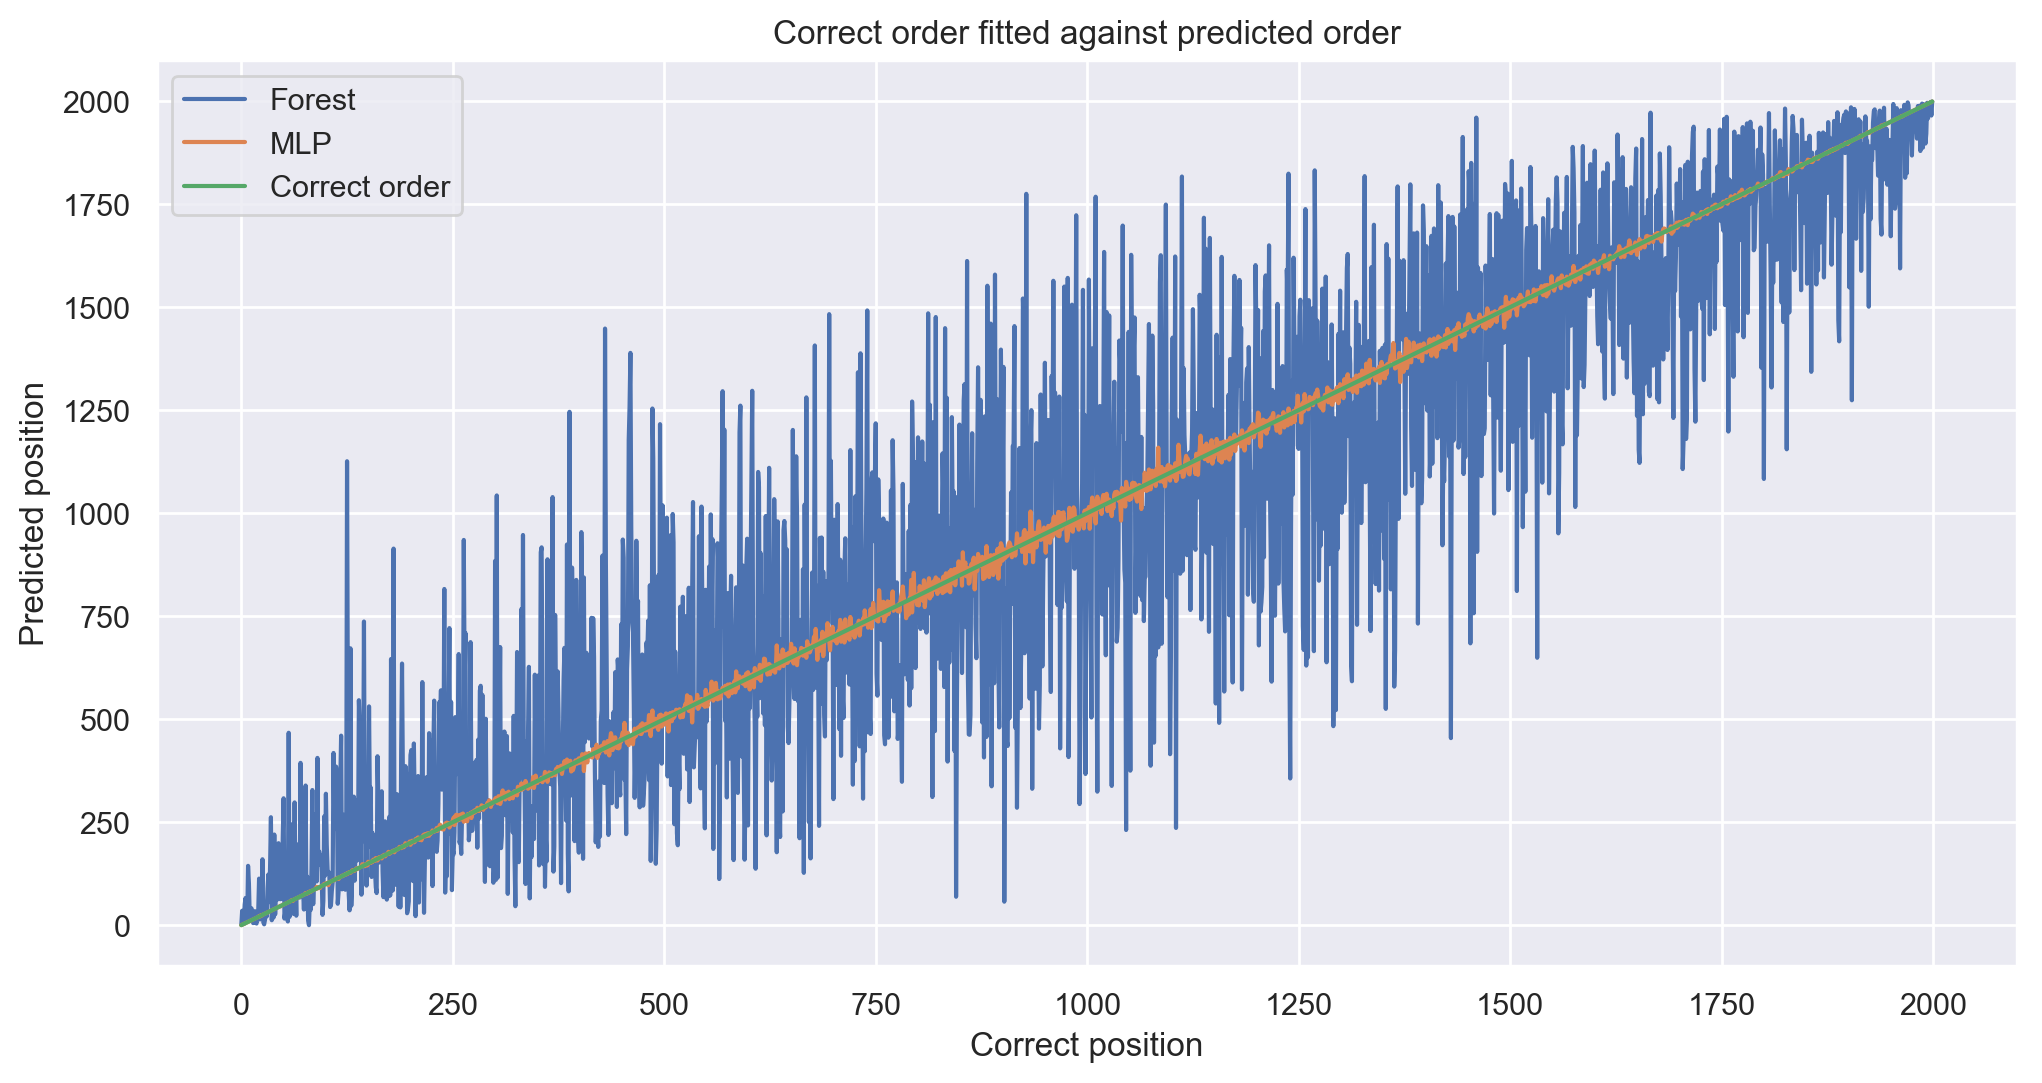
\includegraphics[width=\linewidth]{images/mlp_forest_comparison02.png}
		\caption{\textit{This figure displays the same data as Figure \ref{forest_mlp_comp1}. Here, the x-axis represents the position of each instance sorted by its target value, the y-axis displays the position if the instances had been sorted by the predicted target values of the respective regressor. The more the predictions resemble the correct order (the green line) the better the regressor is suited for our task.}}
		\label{forest_mlp_comp2}
	\end{figure}

	In order to get a feeling for the performance of both regressors, we used the function \code{sklearn.datasets.make\_regression} to create $10000$ samples with $100$ features of which $10$ are informative. We then trained the Random Forest Regressor and the MLP-Regressor with $80\%$ of the generated data and let both regressors predict the values of the remaining $20\%$ of the data. Figure \ref{forest_mlp_comp1} shows how much more accurate the MLP-regressor performs compared to the Random Forest Regressor. Figure \ref{forest_mlp_comp2} shows how the MLP-Regressor maintains the order of the instances much better than the Random Forest Regressor. In case of the latter, many values are sorted into completely other regions than where they actually belong. This is also due to the fact that the range of values of the generated data is of the same magnitude as the inaccuracies of the Forest. Still, the MLP manages to predict these values much better.

	